\chapter{SNMP Monitoring}

MIB-II (RFC 1213) definisce i tipi di oggetto per i protocolli Internet IP, ICMP, UDP, TCP, SNMP (e altre definizioni non rilevanti qui).\
Fondamentalmente modella la gestione dello stack del protocollo TCP/IP.\

In totale 170 tipi di oggetti:\ alcune definizioni MIB si sono rivelate troppo semplici e minime (tabella di instradamento, tabella di interfaccia), alcune definizioni MIB presuppongono un formato di indirizzo a 4 byte, quindi queste tabelle devono essere ridefinite per IPv6.

\noindent Obiettivi della definizione MIB-II:
\begin{itemize}
    \item Gestione di base degli errori e della configurazione per i protocolli Internet.\
    \item Pochi deboli controlli
    \item Evitare informazioni ridondanti nel MIB.
    \item L'implementazione di MIB non dovrebbe interferire con le normali attività di rete.
    \item Nessun tipo di oggetto dipendente dall'implementazione.
\end{itemize}

\section{``system'' Group}

Per leggere il \textbf{gruppo system} è possibile eseguire delle \texttt{get} individuali, oppure usare una \texttt{snmpwalk}:\ permette di leggere tutti gli object identifier che iniziano con un certo prefisso.\
Tutti gli oggetti facenti parte di tale gruppo sono \textbf{scalari}.\

\begin{figure}[H]
    \centering
    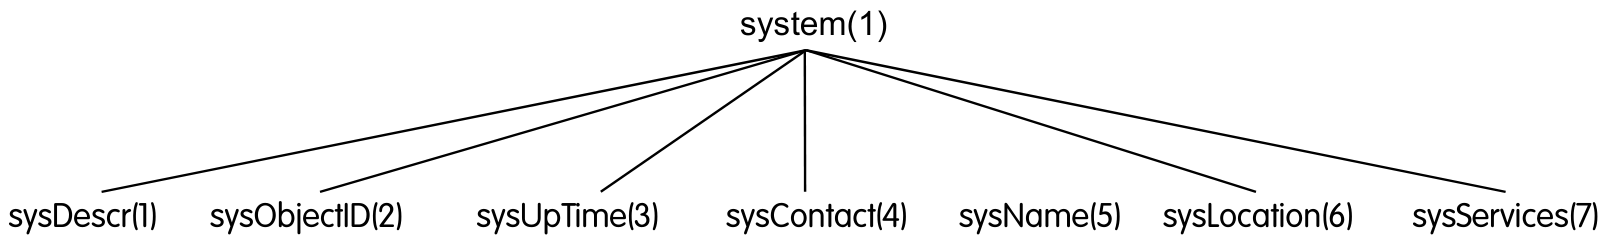
\includegraphics[width=\textwidth]{immagini/system_group.png}
\end{figure}

\begin{itemize}
    \item\texttt{sysDescr}:\ contiene una descrizione approssimata di quello che fa una certa device sottoforma di una stringa libera.
    \item \texttt{sysObjectID}:\ è un object identifier che contiene informazioni riguardo la device (tipicamente contiene informazioni sul costruttore).
    \item \texttt{sysUpTime}:\ tempo di attività dell'agent SNMP, viene usato per determinare le discontinuità del servizio.\ Se $\mathtt{sysUpTime}_{t_1} > \mathtt{sysUpTime}_{t_2}$, dove $t_2 > t_1$, l'agent è stato reinizializzato e l'applicazione di gestione si basa sui valori precedenti.\
    \item \texttt{sysContact}:\ contiene le informazioni per raggiungere il gestore della device.
    \item \texttt{sysName}:\ nome simbolico della device.
    \item \texttt{sysLocation}:\ indica dov'è fisicamente installata la device (la locazione potrebbe non essere aggiornata).
    \item \texttt{sysServices}:\ bitmap che riporta approssimativamente i servizi forniti dal sistema (utile quando non si capisce di che device si tratti usando \texttt{sysObjectID}).
\end{itemize}

\noindent In poche parole, il gruppo \texttt{system} è importante per mappare il dispositivo (tramite \texttt{sysObjectId.0}, \texttt{sysDescr.0} e \texttt{sysLocation.0}), controllare il wrapping check (\texttt{sysUpTime.0}) e segnalare problemi relativi al dispositivo all'amministratore (\texttt{sysContact.0}).

\section{``interface'' Group}

Quando si interroga il gruppo delle interfacce si va a leggere e enumerare lo stato delle interfacce della periferica.

\begin{figure}[H]
    \centering
    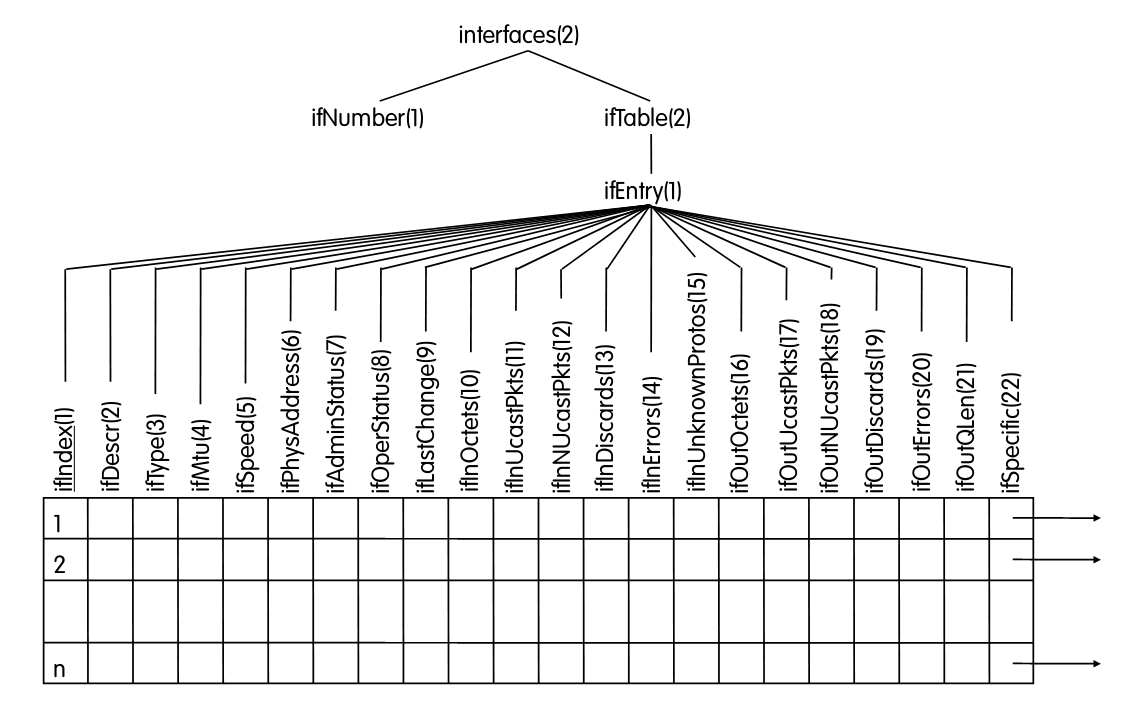
\includegraphics[width=\textwidth]{immagini/interface_group.png}
\end{figure}

\begin{itemize}
    \item\texttt{ifNumber}:\ numero delle interfacce.
    \item\texttt{ifIndex}:\ chiave della tabella.
    \item\texttt{ifDescr}:\ descrizione dell'interfaccia.
    \item\texttt{ifType}:\ tipo dell'interfaccia.
    \item\texttt{ifMtu}:\ MTU massima dell'interfaccia.
    \item\texttt{ifSpeed}:\ velocità dell'interfaccia di rete (in teoria quella reale).
    \item\texttt{ifPhysAddress}:\ MAC address dell'interfaccia.
    \item\texttt{ifAdminStatus}:\ lo stato amministrativo corrente dell'interfaccia.\ Valori:\ \texttt{up} (1), \texttt{down} (2), \texttt{testing} (3).\ Un valore diverso da \texttt{up} significa che l'interfaccia non è fisicamente presente sul sistema o che è presente ma non disponibile per il sistema operativo (per esempio il driver non è stato caricato).\ Caveat:\ SNMP MIB index holes.
    \item\texttt{ifOperStatus}:\ lo stato operativo corrente dell'interfaccia.\ Valori:\ \texttt{up} (1), \texttt{down} (2), \texttt{testing} (3).\ È simile a \verb|ifconfig <device> up/down|.
    \item\texttt{ifOutQLen}:\ la lunghezza della coda dei pacchetti di output (in pacchetti).\ È utile per saperne di più sulle velocità di trasmissione e sul throughput (buffer pieno significa che il destinatario non è veloce come il mittente).
    \item\texttt{ifLastChange}:\ contiene il valore di \texttt{sysUpTime} nel momento in cui l'interfaccia è entrata nel suo stato operativo corrente.\ Utile per rilevare quando un'interfaccia cambia stato (per esempio se viene scollegato un cavo).
\end{itemize}

\begin{figure}[H]
    \centering
    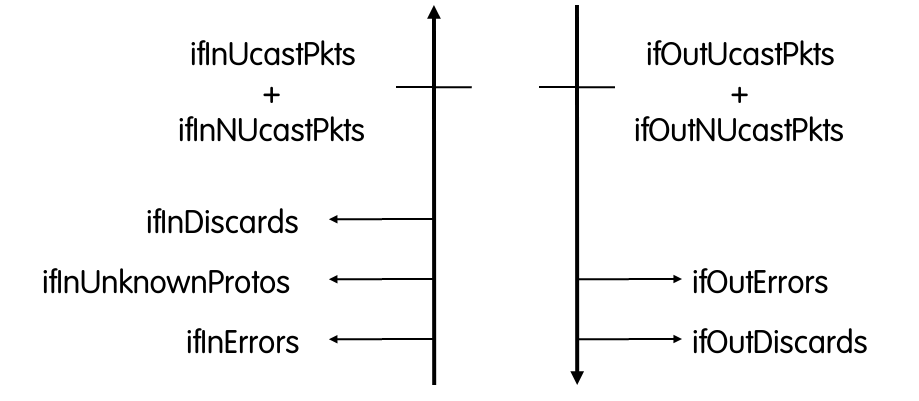
\includegraphics[width=0.7\textwidth]{immagini/interface_group_diagram.png}
\end{figure}

\noindent I diagrammi dei casi illustrano le dipendenze tra le variabili:\ il numero di pacchetti forniti da un'interfaccia di rete al successivo livello di protocollo superiore: \[\mathtt{ifInUcastPkts} + \mathtt{ifInNUcastPkts}\]
il numero di pacchetti ricevuti dalla rete:
\begin{center}
    (\texttt{ifInUcastPkts} + \texttt{ifInNUcastPkts}) + \texttt{ifInDiscards} + \texttt{ifInUnknownProtos} + \texttt{ifInErrors}
\end{center}
il numero di pacchetti effettivamente trasmessi:
\begin{center}
    (\texttt{ifOutUcastPkts} + \texttt{ifOutNUcastPkts}) - \texttt{ifOutErrors} - \texttt{ifOutDiscards}
\end{center}

\subsubsection{Usare il gruppo ``interface''}

È la base del monitoraggio basato su SNMP:\ molti strumenti eseguono periodicamente il polling dei valori dalle interfacce (principalmente \texttt{ifInOctets} e \texttt{ifOutOctets}).\

I valori sono aggregati e non divisi per protocollo, destinazione o AS; questa è una limitazione importante se è richiesto un monitoraggio a grana fine.\
Il motivo è che i contatori SNMP sono fondamentalmente i contatori del kernel ``esposti'' tramite SNMP.\
Gli errori di interfaccia possono essere utilizzati per rilevare problemi di comunicazione, in particolare sui collegamenti WAN.\

Le statistiche sulla dimensione dei pacchetti non vengono riportate, tuttavia è possibile calcolare semplici statistiche sugli ottetti/pacchetti.\
Molti produttori (ad esempio Cisco, Juniper) segnalano informazioni sulle interfacce fisiche e logiche (note anche come interfacce secondarie), altri (es.\ Extreme) hanno la voce nella tabella ma i contatori sono sempre zero.\
Utilizzando i contatori dell'interfaccia è possibile produrre report su:
\begin{itemize}
    \item VLAN (LAN virtuale),
    \item PVC (circuito virtuale privato) sui collegamenti Frame Relay.
\end{itemize}

\section{Uso del gruppo ``arp''}

Utile per accedere alla tabella arp (Address Resolution Protocol) di un dispositivo remoto.\
Può essere utilizzato per identificare attacchi di arp-poisoning o host configurati in modo errato (ad esempio indirizzi IP duplicati).

\section{Bridge MIB}

Utile per controllare lo stato degli interruttori L2/L3, non viene usato solo sui bridge.\
È in qualche modo complementare al MIB II in quanto fornisce informazioni agli host collegati alle porte dello switch.\
Usi comuni del bridge MIB:
\begin{itemize}
    \item Per conoscere l'indirizzo MAC di un host collegato alla porta X/unità Y dello switch \texttt{dot1dTpFdbTable.dot1dTpFdbAddress} (\textbf{Nota}:\ il MIB II ha l'indirizzo MAC della porta dello switch).
    \item L'associazione MAC/porta è la base per rilevare la posizione fisica di un host.\ In effetti, poiché le porte dello switch sono solitamente collegate alle prese a muro, questo è un buon metodo per sapere chi è dove (utente $\rightarrow$ computer $\rightarrow$ porta dello switch $\rightarrow$ stanza/scrivania).
    \item Mantiene traccia dell'indirizzo MAC ``precedente'' (e dell'ora) connesso a una porta in modo che sia possibile tenere traccia degli utenti mentre si spostano da una stanza all'altra.
    \item Può essere utilizzato per rilevare le porte con più indirizzi MAC associati (trunk), quindi per rilevare utenti con più MAC (ad esempio un utente esegue VMware sul proprio PC o un utente è stato infettato da un virus/worm) o porte con uno switch collegato ad esso che la politica di rete potrebbe essere violata.
\end{itemize}

\noindent Con il Bridge MIB è possibile sapere dove sono attestati i MAC address (a patto che un nodo supporti SNMP), ma non permette di conoscere la \textbf{topologia} della rete; per fare ciò è possibile utilizzare il \textit{Link Layer Discover Protocol} (\textit{LLDP}):\ permette di sapere a quale porta è fisicamente un'altra porta.\
LLDP si basa su messaggi Ethernet.\

\section{SNMP vs.\ CLI Counters}

È opinione comune tra la comunità degli amministratori di rete che i contatori SNMP e CLI siano fondamentalmente una visione diversa della stessa cosa.\
A molti amministratori piacciono di più i contatori CLI, in quanto sono formattati per essere più comprensibili agli umani e molte implementazioni forniscono il comando per cancellare/azzerare il contatore.\
Si noti che la definizione di ciò che conta un dato contatore dipende dalla documentazione del fornitore.

I contatori CLI rimangono lo stile di vita di base nella gestione degli elementi.\
Il formato/aspetto dei contatori cambia da fornitore in fornitore, spesso anche all'interno dello stesso produttore come Cisco IOS, CatOS e PIX (sono rispettivamente il router, lo switch e il firewall OS utilizzati dai dispositivi Cisco).\

I contatori SNMP invece permettono di ``confrontare le mele con le mele'':\ i contatori hanno definizioni standard (definite da IETF, IEEE, alcuni fornitori\dots) indipendentemente dal tipo di elemento di rete o dal fornitore e dai nomi univoci a livello globale e difficili da pronunciare.\
Hanno una dimensione ben specificata, 32 o 64 bit (64 bit disponibile in SNMP v2c o v3), non iniziano necessariamente da zero e non sono progettati per essere usati direttamente dagli umani:\ richiedono una funzione delta per calcolare la velocità.\

\textbf{Nota}:\ i buoni contatori sono generalmente derivati dalla specifica del protocollo sottostante.

\subsubsection{Calcolare l'utilizzo della larghezza di banda con SNMP}

Bandwidth Utilisation

\[
    \frac{(\mathtt{\Delta ifInOctets + \Delta ifOutOctets}) \times 8 \times 100}{\mathit{\Delta time \times speed}}
\]

\noindent Input Utilisation:\ $\mathtt{\Delta ifInOctets} \times 8 \times 100/(\mathit{\Delta time \times speed})$

\noindent Output Utilisation:\ $\mathtt{\Delta ifOutOctets} \times 8 \times 100/(\mathit{\Delta time \times speed})$

\subsubsection{Cos'altro può fare SNMP?}

\begin{itemize}
    \item Rilevare e cancellare le connessioni TCP bloccate.
    \item Manipolare le voci ARP.
    \item Ottienere la temperatura ambientale.
    \item Controllare l'utilizzo della CPU.
    \item Monitorare gli alimentatori ridondanti/uninterruptible.
    \item Trovare utenti P2P (tabella NAT).
    \item Layout di topologia di rete (ad es.\ tramite CDP).
\end{itemize}

\section{RMON:\ Remote Monitoring}

Presente nella maggior parte delle apparecchiature di rete di fascia medio-alta, spesso si tratta di implementazioni scarse/limitate.\
Alcuni fornitori vendono sonde autonome:\ caso preferito in quanto sono implementazioni complete del protocollo e non aggiungono ulteriore carico al router.\
Non tutte le implementazioni (in particolare quelle incorporate in router/switch) supportano l'intero standard ma solo gruppi SNMP selezionati.\

Insieme a Cisco NetFlow è lo standard di monitoraggio industriale ``affidabile''.\
Due versioni: RMON-1 (L2) e RMON-2 (L2/L3).

\begin{center}
    \textit{Cosa può fare RMON}?
\end{center}

\begin{itemize}
    \item Raccogliere i dati e segnalarli periodicamente a una stazione di gestione più centrale, che potenzialmente riduce il traffico sui collegamenti WAN e il sovraccarico di polling sulla stazione di gestione.\
    \item Indicare quali host sono collegati alla LAN, quanto parlano e con chi.
    \item ``Visualizzare'' tutto il traffico LAN, utilizzo completo della LAN e non solo il traffico verso o attraverso il router.
    \item Filtrare e catturare i pacchetti (in modo da non dover visitare una LAN remota e collegare un analizzatore di LAN):\ è fondamentalmente uno sniffer remoto in grado di catturare il traffico in tempo reale (fino a quando il buffer di memoria integrato non è pieno).
    \item Raccogliere automaticamente i dati, confrontarli con le soglie e inviare \texttt{trap} alla stazione di gestione:\ ciò scarica gran parte del lavoro che potrebbe impantanare la stazione di gestione.
\end{itemize}

\subsubsection{RMON vs. SNMP}

Il protocollo SNMP viene utilizzato per controllare e configurare una sonda.\
Di solito i gestori GUI mascherano la complessità della configurazione basata su SNMP.\
Le statistiche e il traffico salvato vengono recuperati utilizzando SNMP dalle applicazioni di gestione per registrare statistiche su una rete e, eventualmente, porzioni selezionate del traffico di rete.

SNMP e RMON differiscono nel modo in cui raccolgono le statistiche sul traffico:\ SNMP esegue periodicamente delle richieste (polling) per ottenere le statistiche di rete (lo stato della rete è mantenuto dal gestore); RMON, d'altra parte, riduce lo stress del manager raccogliendo e archiviando le statistiche in contatori o \textit{bucket} per il recupero da parte di una stazione di gestione.\

%rmon groups

\subsubsection{Utilizzo della rete con RMON}

La maggior parte dei gestori RMON utilizza i contatori RMON per calcolare l'utilizzo della rete.\
L'utilizzo della rete può essere calcolato per tutte le porte di un determinato switch a intervalli regolari.\

Queste informazioni possono essere raccolte nel corso della giornata e utilizzate per generare un profilo di utilizzo della rete di uno switch o hub.
\[ \%\ \mathrm{Network\ Utilisation} = \frac{100 \times ((\#\mathrm{packets} \times 160)+ (\#\mathrm{octets}\times 8))}{\mathrm{port\ speed \times time(sec)}}\]

\subsubsection{RMON Alarm Group}

Viene prodotto un evento ogni volta che viene superata una soglia, oppure quando un valore che prima era al di sopra di tale soglia ritorna all'interno dell'intervallo specificato.\
Considerazioni simili possono essere applicate a un valore di soglia inferiore.\

Le soglie possono essere sul valore misurato (assoluto) o sulla differenza tra il valore corrente e l'ultimo valore misurato (valore delta).
